\label{fs-formalism}

\subsection{Distributed streaming model}

\begin{definition}{Reference stream processing system}
is a tuple of $(\Gamma,D,W^{*}_{\tau+1}(W^{*}_\tau))$. $\Gamma$ is a set of all possible data flow elements. $D\subseteq{2^{\Gamma}\times2^{\Gamma}}$ is a binary relation on it. Pair $(x,y)\in{D}$ if $y$ can be generated from $x$ within user-defined operations. We assume that all operations are pure and that it is possible to construct transitive closure of $D$. $W^{*}_{\tau+1}(W^{*}_\tau)$ is a processing rule, where on each iteration next step is randomly chosen:\\

$W^{*}_0=\emptyset$:

$W^{*}_{\tau+1}=\begin{sqcases}
W^{*}_{\tau}\cup{a_{\tau+1}},a_{\tau+1}\in{\Gamma} & \text{or}\\
W^{*}_{\tau}\setminus{b_{\tau+1}}, b_{\tau+1}\in{2^{\Gamma}}, & \text{or}\\
W^{*}_{\tau}\setminus{X}\cup{Y}, (X,Y)\in{D} & \text{}.
\end{sqcases}$

\end{definition}

In a classical model proposed by Chandy and Lamport~\cite{Chandy:1985:DSD:214451.214456}, a distributed system is represented as a graph of processes, which can be connected to each other via channels. Each process can own a modifiable internal state, generate {\em events} and send them to other processes through the channels. {\em Global system state} in this model contains processes states and channel states, e.g., elements, which are in-flight at the moment. Distributed asynchronous processing is simulated using permutations of events.

The proposed model is a variation of a classical Chandy-Lamport distributed system model with the following properties and modifications:

\begin{itemize}
    \item Input and output elements $a_\tau$ and $b_\tau$ are special events. In most state-of-the-art stream processing systems, end-user is external to the system, i.e., a user is able to observe input and output elements, but not the system states.
    \item Our notion of a streaming system does not provide a concept of {\em operations state} because as it is shown in~\cite{we2018adbis}, states can be considered as ordinary data items. In this case, a state element is presented in a system until it is transformed into a new state together with new elements. Hence, $W_\tau$ is a global state with only channel states in terms of Chandy-Lamport.
    \item $D$ captures distributed asynchronous computations within a graph of processes that is a physical streaming execution graph in our case. 
\end{itemize}

We can imagine a stream processing system as a pool, where some elements are poured in and others are poured out. Inside a pool, each element can be transformed into the other element, which can be transformed as well, and so on. Only survived elements are poured out from the pool. 

Within our model, one can define a streaming system using only data flow elements and operations. $\tau\in{\mathbb{N}}$ can be considered as an exact global discrete time. We assume that only one event can happen at any single point in time $\tau$. $a_\tau\in{\Gamma}$ is the element, which enters at the time $\tau$, and $b_\tau\in{2^\Gamma}$ are the elements, which leave at the time $\tau$. 

Let $A_{\tau}=\{a_i\}^{\tau}_{i=1}$ be a set of all input elements by the time $\tau$ and ${B}_\tau=\bigcup\limits_{i=1}^{\tau}{b_i}$ be a set of all output elements. $b_\tau$ is a set because some elements must be released atomically. Since end-user typically cannot observe internal transitions directly, it is convenient in some cases to limit the global time domain only to moments of output events.

\begin{definition}{Time quantization}
$\tau(t)$ is monotonic mapping from time domain restricted to only output events to global discrete time $\tau$, $\forall{t}\exists{b_{\tau(t)}}$.
\end{definition}

\begin{definition}{Probability of output element in a reference system}
$P(b_{t+1}|A_{t+1}, B_t)$ is a probability to observe output set $b$ at the time $t+1$ considering all previous input and output elements. For all output elements from the reference working set, such probability is positive,\\
$\forall{b_{t+1}:\exists{W^{*}_{t+1}=W^{*}_{t}\setminus{b_{t+1}}}} \Rightarrow P(b_{t+1}|A_{t+1}, B_t) > 0$.
\end{definition}

The reference stream processing system is just an abstract concept because it does not capture possible failures of network and computational units. Failure can be expressed as a loss of the working set or its part. There is a need to extend the reference model by a recovery mechanism that allows a system to transparently pass through the failures.

% {\bf Snapshot = set!}
% P and P_{\tau}??

\begin{definition}{Stream processing system}
is a tuple of\\
$(\Gamma,D,W_{\tau+1}(W_\tau),P,F)$. As in a reference system, $\Gamma$ and $D$ define the possible data items and user-defined computations. Snapshot $P$ is an information about system execution that is available even in case of a system failure. At time $\tau$ snapshot contains information $P_\tau$. Recovery function $F(A^{p}_\tau,P_\tau)$ provides logic for recovering of working set in case of system failures based on some set of input elements $A^{p}_\tau\subseteq{A_\tau}$ and a snapshot $P_\tau$. Processing rule $W_{\tau+1}(W_\tau)$ is extended with a {\em recovery transition}:

$W_0=\emptyset$:

$W_{\tau+1}=\begin{sqcases}
W_{\tau}\cup{a_{\tau+1}}, & \text{or}\\
W_{\tau}\setminus{b_{\tau+1}}, & \text{or}\\
W_{\tau}\setminus{X}\cup{Y}, \forall{x\in{X}\exists{y\in{Y}}}:(x,y)\in{D} & \text{or}\\
F(A^{p}_\tau,P_\tau), A^{p}_\tau\subseteq{A_\tau} & \text{}.
\end{sqcases}$

\end{definition}

\begin{definition}{Probability of output element}
$P(b_{t+1}|A_{t+1}, B_t, P_t,F)$ is a probability to observe output element $b$ at the time $t+1$ considering all previous input and output elements, current snapshot, and recovery function.
\end{definition}

\subsection{Consistency guarantees}

The reference system concept allows us to express the notion of valid execution in terms of correspondence between input and output elements. In most real cases, input and output elements are the only data that can be observed by end-user. In real distributed stream processing systems, failures and recoveries can corrupt the output, despite the fact, that in terms of a naive definition of delivery guarantees, all elements are processed exactly once. Let us demonstrate it by an example. Assume that execution graph consists of a single operation $V^{i+1}=a_\tau(1+V^{i}),V^{0}=0,V\in{S}$ and $\forall{t},b_t=V$. In case of failure and recovery, the consistency of subsequent results depends not only on further input elements but on the restored $V$ as well. If a system recovers $V$ incorrectly after a failure, the results may become inconsistent, e.g. the property of output monotonicity can be violated. For instance, if $V=0$ after recovery, but before failure it was equal to some value $q\neq{0}$, end-user will receive unexpected output, even if each input element $a_\tau$ is processed exactly once. This example is demonstrated in Figure~\ref{state-inconsistency}. 

\begin{figure}[htbp]
  \centering
  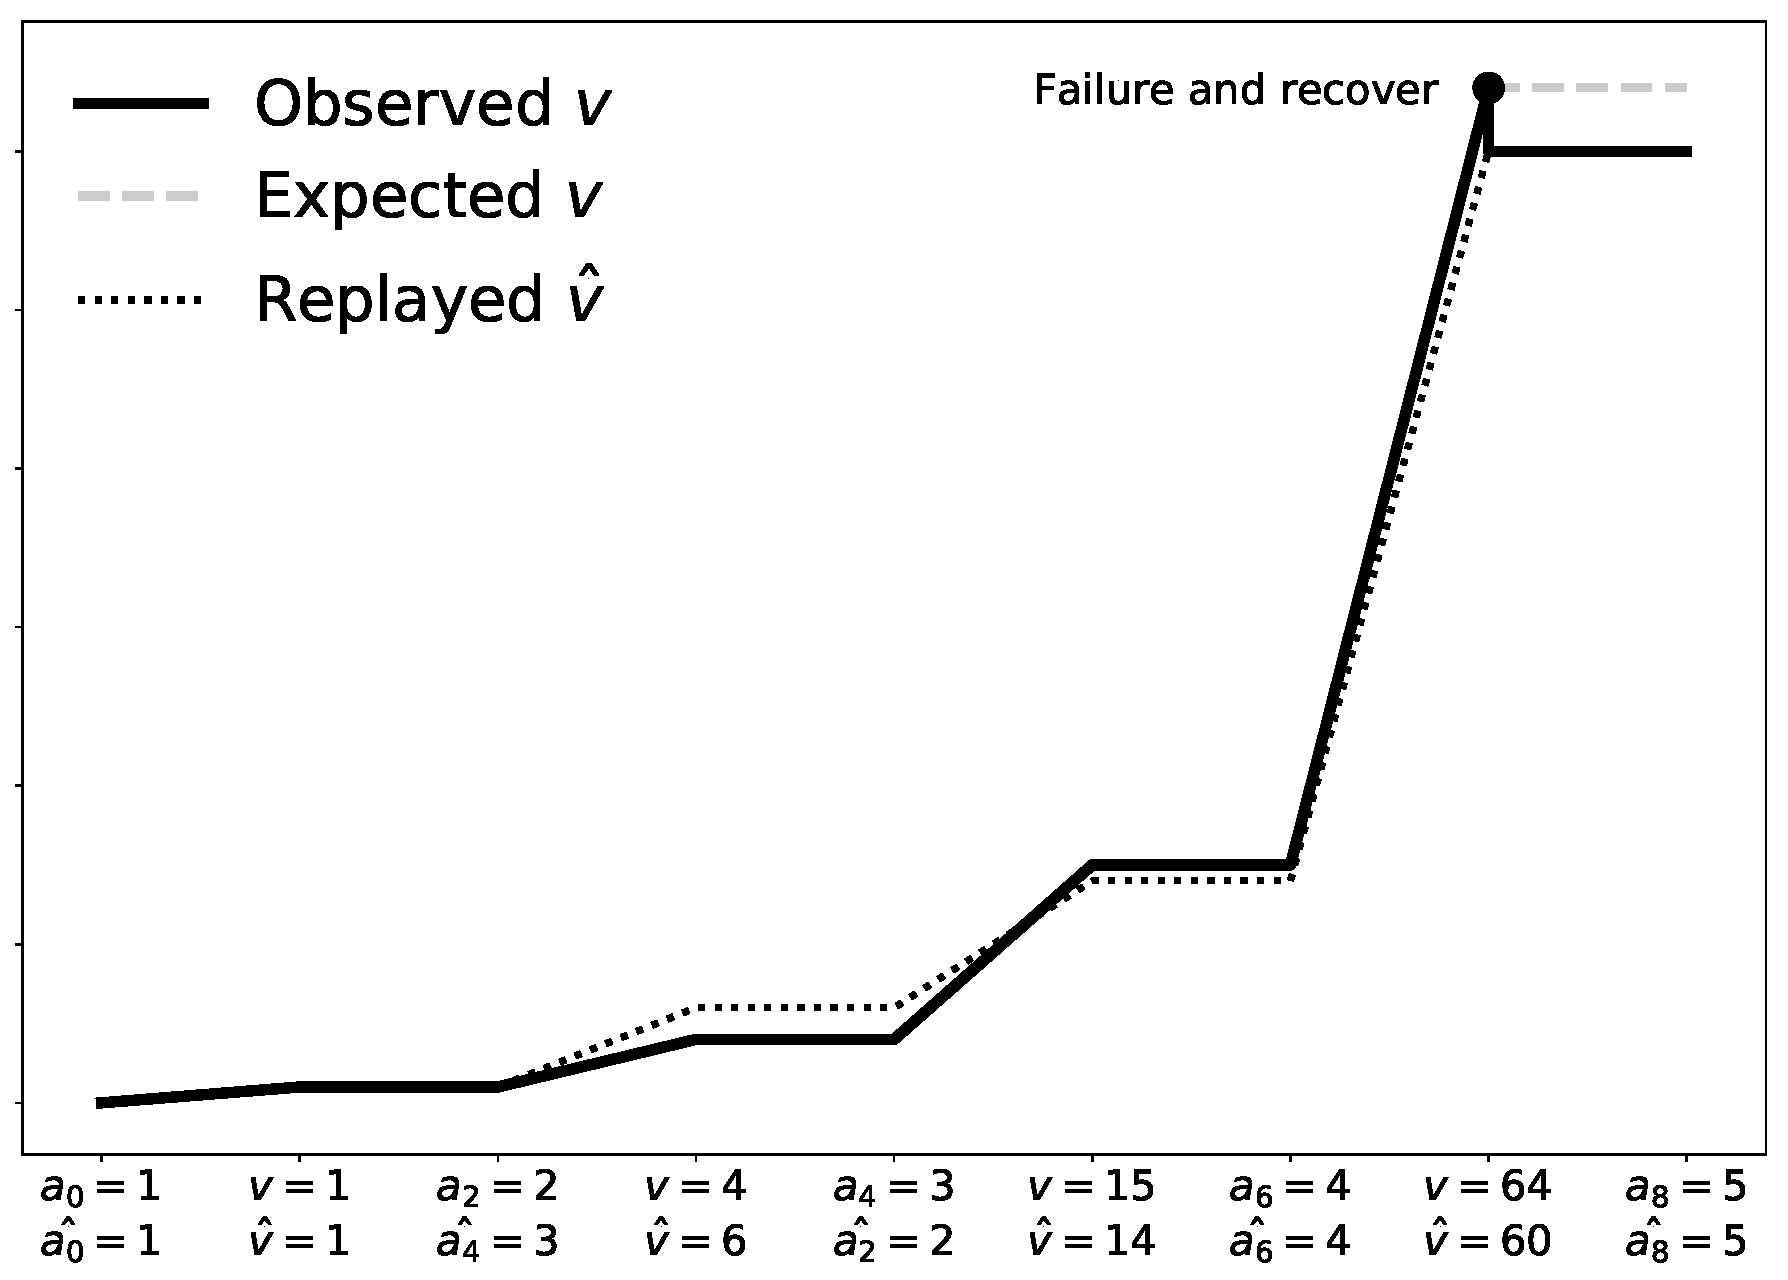
\includegraphics[width=0.48\textwidth]{pics/failure}
  \caption{Inconsistency of results after incorrect recovery}
  \label {state-inconsistency}
\end{figure}

\begin{definition}{System provides for exactly once}
if it is possible to obtain each output element $b_{t+1}$ in the reference stream processing system, i.e.,\\ 
$\forall{t} \forall{b_{t+1}}: P(b_{t+1}|A_{t+1},B_t,P_t,F)>0 \Rightarrow P(b_{t+1}|A_{t+1},B_t)>0$.
\end{definition}

\begin{definition}{System provides for at most once}
if \\
$\exists{A^{0}_{t+1}\subseteq{A_{t+1}}}$ such that \\
$\forall{t} \forall{b_{t+1}}: P(b_{t+1}|A_{t+1},B_t,P_t,F)>0 \Rightarrow P(b_{t+1}|A^{0}_{t+1},B_t)>0$.
\end{definition}

\begin{definition}{System provides for at least once}
if \\
$\exists{A^{*}_{t+1}\subseteq{2^{A_{t+1}}}}$ such that \\
$\forall{t} \forall{b_{t+1}}: P(b_{t+1}|A_{t+1},B_t,P_t,F)>0 \Rightarrow P(b_{t+1}|A^{*}_{t+1},B_t)>0$.
\end{definition}

Exactly once states that observed results cannot be distinguished from one of the possible results produced by the reference system. At most once and at least once guarantees are the relaxations of exactly once. The results within these guarantees can be obtained in the reference system, but with the assumption, that input is not completely correct. At least once can be reproduced if the input contains duplicates. At most once can be achieved in the reference system if some input elements are missed. It is important to note, that regarding at most once guarantee we require an input element to be processed atomically with all its derivatives or not processed at all. To the best of our knowledge, no one real stream processing engine supports at most once guarantee, so we cannot verify the relevancy of this assumption. It is easy to provide at most once by producing no output at all but if the output is presented, at most once enforcement becomes much more difficult.  

In our formal model, the relaxations of exactly once are defined without diving into recovery mechanisms. Instead, they are described through possible input channel flaws in a reference system. This trick allows us to represent invisible system details in terms clear for a user.

Operations that are presented in $D$ can directly affect the complexity of consistency enforcement mechanisms. For example, if all operations are idempotent, exactly once can be obviously achieved~\cite{Akidau:2013:MFS:2536222.2536229}. On the other hand, if the system supports a variety of operations including non-idempotent and non-commutative, exactly once becomes challenging.

\begin{definition}{System is deterministic}
if\\ 
$\forall{t\in{\mathbb{N}}, b_{t+1}\in{2^{\Gamma}}}:P(W_{t+1}|A_{t+1},B_t)=1$.
\end{definition}

An important property of a deterministic system is that it preserves the same order of elements before non-commutative operations on each run.

\begin{theorem}
\label{necessary_conditions}
If system is non-deterministic and $D$ captures at least one non-commutative operation then system must atomically release all descendants of an input element in order to preserve exactly once.
\end{theorem}
\begin{sketch}
$ $\newline
Let $a_\tau$ be an input element and $x_1,x_2 \in Cl(D)(a_\tau)$. Let $s \in Cl(D)(x_1) \cap Cl(D)(x_2)$ be an element that is obtained through non-commutative operation. Let $b_{t-1},b_{t}\in{Cl(D)(s)}$ be non-atomically released output elements. Assume that system fails at time $\tau(t-1) < \tau_f < \tau(t)$. There are two possible recover behaviors: replay input element $a_\tau$ or not to replay it. The second case is simple: if system decides not to reprocess element $a_\tau$ then $b_t$ will never be obtained and delivered that is an obvious contradiction to consistent recovery. If system reprocesses $a_\tau$, element $s$ may become different than before replay due to non-commutative operation and possible reorderings in asynchronous and distributed environment. Let us denote it as $s'$. Therefore, after recovery element $b_t$ will be delivered, but it will depend not on $s$, but on $s'$: $b_t\in Cl(D)(s')$. This is a contradiction, because $b_t$ has been already delivered and $P(b_{t}\in Cl(D)(s')|\{a_\tau\},\{b_{t-1} \in Cl(D)(s) \})=0$.
\end{sketch}

In the proposed theorem, we assume that input element $a_\tau$ is split into elements $x,y$. The same proof can be obviously achieved under the assumption of two input elements $a_\tau$ and $a_{\tau+1}$ which enter a system through asynchronous channels.

\begin{corollary}
If system is non-deterministic and $D$ captures at least one non-commutative operation then system must atomically take snapshot and release all descendants of an input element in order to preserve exactly once.
\end{corollary}
\begin{sketch}
$ $\newline
Let us do all assumptions from the Theorem~\ref{necessary_conditions}. Let us suppose that $s$ is an operation state that system includes in a snapshot. Therefore, $s \in W_t$ after a recovery. By the formula of total probability,

$P(b_{t}|A_{t},B_{t-1})=\\
\sum\limits_{W_{t}}P(W_{t}|A_{t+1},B_{t-1})P(b_{t}|A_{t},B_{t-1},W_{t})=\\
\sum\limits_{W_{t}}P(W_{t}|A_{t+1},B_{t-1})P(b_{t}|W_{t}) > 0
$,

working set $W_{t+1}$ must also be consistent with previous input and output elements to enforce exactly once. Hence, $s$ can be considered as an ordinary output element, and must be saved atomically with releasing of  because of the fact that $s\in Cl(D)(a_\tau)$.
\end{sketch}

This theorem has a direct practical implication. If a system aims at providing for exactly once, it must output elements $b_t$ only if there exists a snapshot for time $t$. It means that the lower bound of latency in the worst case in such systems is the snapshotting period together with the duration of taking a snapshot. There is a trade-off between latency and the frequency of taking snapshots because too frequent snapshotting can cause high extra load, while rare snapshots lead to high latency.

\begin{corollary}
If the system is deterministic and $D$ captures non-commutative operations then the system can take a snapshot and release all descendants of an input element non-atomically while preserving exactly once.
\end{corollary}
\begin{sketch}
$ $\newline

Let us do all assumptions from the Theorem~\ref{necessary_conditions}. In case of a deterministic system, it is guaranteed that $s=s'$. 
\end{sketch}

If a system is deterministic, it is possible to inexpensively achieve a consistent snapshotting mechanism without synchronization between taking snapshots and output elements delivery. Deterministic system can release an element $b_t$ before snapshot $P^{s}_t$ at time $t$ is taken. As we show further in experiments, this relaxation is able to dramatically decrease processing latency, because there is no need to wait until the snapshot is taken in order to release output elements.

To the best of our knowledge, only micro-batching systems support the property of determinism in streaming. However, micro-batching solutions provide higher latency than pure streaming engines due to overhead on input buffering~\cite{karimov2018benchmarking}. We proposed a pure streaming model called {\em drifting state}~\cite{we2018adbis} that allows achieving both determinism and low latency. Therefore, a question arises: is it more efficient in practice to handle non-determinism by atomic snapshotting and releasing than to maintain a fair determinism in order to get exactly once? 

It is important to note that the proposed model is suitable not only for the formal analysis of the properties of exactly once but for a deeper understanding of the other aspects of stream processing. While these topics are promising as well, they are out of the scope of this paper. 

\subsection{Examples}

In state-of-the-art stream processing systems $\Gamma$ contains all possible objects that can be processed inside a system. For example, in Storm, $\Gamma$ contains all possible {\em Tuples}, while in Flink all {\em StreamRecords}. Dependency relation $D$ is defined in a form of a logical graph that is commonly assumed as directed and acyclic.

\subsubsection{MillWheel}

MillWheel maintains the whole $W$ in a snapshot. Each operation saves all its input elements for deduplication and output elements for resending. There is no need to replay input elements because the system can completely restore computations using only a snapshot. {\em Strong productions} mechanism allows MillWheel to preserve exactly-once guarantee for the price of persistent updates of $P_\tau=W_\tau$ on each $\tau$~\cite{Akidau:2013:MFS:2536222.2536229}.    

\subsubsection{Flink}

Flink uses the state snapshotting mechanism. It artificially reproduces a moment $t_s$, when $\forall{a}\in{Cl^{-1}(D)(S_{t_s})}:\theta_a \leq t_s$, and saves obtained $S_{t_s}$. Flink achieves consistent state by injecting special elements called {\em checkpoints} into the input stream. Checkpoints go through the same network channels as ordinary elements and push all inverted dependencies of inputs through the system. Each operation in data flow prepares its snapshot independently at the moment of checkpoint arrival. Global snapshot is taken when checkpoint passes through the whole data flow. Flink atomicity between state snapshotting and elements delivery is preserved using the modification of 2PC protocol.

Besides overhead on snapshotting and delivery synchronization, checkpoints cause extra latency overhead because an operation with multiple inputs must wait until checkpoints arrive from each input. Only after that, an operation can safely send checkpoint further. This behavior is known as {\em checkpoints alignment}.

\subsubsection{Spark streaming}

To the best of our knowledge, spark streaming is the only state-of-the-art stream processing system that provides for deterministic results. However, an architecture based on input buffering makes it hard to achieve latency lower than several seconds~\cite{7530084, 7474816}. 
